\documentclass[a4paper, 12pt]{scrartcl}
% A4 Papier, 12pt Schriftgröße
% scriptartcl, weil article für englischsprachigen Raum optimiert



% --- EINSTELLUNGEN FÜR DEUTSCHE DOKUMENTE:
\usepackage[ngerman]{babel}
% new german (neue deutsche Rechtschreibung)

\usepackage[utf8]{inputenc}
% utf8-Eingabe (Umlaute etc...)

\usepackage[T1]{fontenc}
% damit im erstellten PDF auch nach Wörtern mit Umlauten gesucht werden kann

\usepackage{csquotes}
% für deutsche Anführungsstriche

\usepackage[addtotoc]{abstract}


\usepackage{graphicx}
% für Bilder

\title{End-to-end-Learning Ansatz für autonomes Fahren im Miniatur Wunderland}
\author{Nils-Ole Bickel, Michel Brüger}
\date{\today}

\begin{document}
	
\maketitle
% Erstellt den Titel, entsprechend den Angaben in der Präambel

\begin{abstract}
Das Ziel dieses Artikels ist die Beschreibung des Vorgehens bei dem Versuch eine auf \emph{Machine Learning} basierende Lösung für ein Fahrzeug zu entwickeln das sich autonom durch das \emph{Miniaturwunderland} bewegen können soll.

Es wird die verwendete Hardware beschrieben, die darauf verwendete Software, sowie auch der Aufbau und das Training des Netzes, welches durch Ende-zu-Ende-Lernen selbständig den der aktuellen Fahrsituation angepassten Lenkwinkel wählen soll.

Auf das Fahrzeug selbst wird nicht näher eingegangen, lediglich auf die Kamera- und Sensordaten welche von diesem empfangen werden.
	
\end{abstract}

\newpage	

\tableofcontents
% Automatisch erstelltes Inhaltsverzeichnis
% zweimal kompilieren, damit Änderungen korrekt angezeigt werden

\newpage
% neue Seite anfangen, damit Titel und Inhaltsverzeichnis auf eigener Seite stehen
	


	\section{Hardware}
		\subsection{Raspberry Pi 4}
		Die Hardware in dem Fahrzeug selbst ist nicht stark genug um aus den Kamerabildern den entsprechenden Lenkwinkel zu berechnen. Daher ist das Ziel, die Berechnung der Lenkwinkel auszulagern, auf einen Rechner, der im besten Fall unauffällig im \emph{Miniaturwunderland} "getarnt" werden kann. 
		
		Der \emph{Raspberry Pi 4} hat im Verhältnis zu seiner Größe potente Hardware und verfügt vor allem auch über zwei USB-3-Anschlüsse. Diese sind wichtig um das volle Potential aus dem \emph{Google Coral USB Accelerator} herauszuholen. Außerdem bietet er die Möglichkeit vollwertige Linux-Betriebssysteme zu installieren, was die Verwendung der für die AI-Lenkwinkel-Voraussagung notwendigen Software ermöglicht.
		
		Die Möglichkeit, den \emph{Raspberry Pi} über eine Powerbank per USB-C zu laden, macht es noch leichter ihn in der Kulisse zu verstecken, da man nicht noch ein Kabel zu einem Stromanschluss verlegen muss.
		
		
		\subsection{Google Coral USB Accelerator}
		Der \emph{Google Coral USB Accelerator} ist ein Tensor-Prozessor in Form eines USB-Sticks, der an einen Rechner wie den \emph{Raspberry Pi} angeschlossen werden kann, um die Machine Learning Operationen schnell und besonders energieeffizient durchzuführen. Dies kann der \emph{Raspberry Pi 4} zwar auch alleine bewerkstelligen, der \emph{Google Coral USB Accelerator} ist dabei aber deutlich schneller. Bei spontanen Vergleichen konnten wir eine 14-fache Geschwindigkeit bei der Objekterkennung in Bildern feststellen.

	
		\subsection{Der Trainingsrechner}
		Das Netz wurde auf einem der Laborrechner trainiert. Dieser verfügt über eine \emph{Nvidia Geforce GTX 1050 Ti} Grafikkarte, welche den Trainingsprozess deutlich beschleunigt, im Vergleich zum Training mit der CPU.	
	
	\section{Software}
		\subsection{Auf dem Raspberry Pi verwendete Software}
			\subsubsection{Raspbian}
			Als Betriebssystem auf dem \emph{Raspberry Pi 4} wird \emph{Raspbian Buster} verwendet. Dabei handelt es sich um eine auf Debian basierende Linux-Distribution.
			
			
			\subsubsection{Python}
			Standardmäßig ist \emph{Python 3.7} in \emph{Raspbian Buster} enthalten. Dies ist für die Verwendung des \emph{Google Coral USB Accelerator} mit \emph{Tensorflow Lite} ausreichend.
			
			\subsubsection{Edge TPU runtime}
			Die \emph{Edge TPU runtime} wird für die Kommunikation mit dem \emph{Google Coral USB Accelerator} benötigt.
			
			Während der Installation der \emph{Edge TPU runtime} kann man auswählen, ob man den \emph{Google Coral USB Accelerator} mit Standardgeschwindigkeit oder maximaler Geschwindigkeit (2x Standard) betreiben möchte. Da sich bei unseren Versuchen mit Standardgeschwindigkeit herausgestellt hat, dass der \emph{Raspberry Pi 4} bei der Vorbereitung der Bilder überhitzt, ist eine Installation mit maximaler Geschwindigkeit überflüssig.
			
			\subsubsection{Tensorflow Lite Library für Python}
			Da auf dem \emph{Raspberry Pi 4} lediglich \emph{Tensorflow Lite} Modelle ausgeführt werden sollen reicht die Installation des \emph{Tensorflow Lite interpreter} anstelle aller Tensorflow Pakete.
			
				
		
		\subsection{Auf dem Trainingsrechner verwendete Software}
		Auf den Labor-PCs ist \emph{Anaconda} installiert.
			\subsubsection{Anaconda}
			In \emph{Anaconda} können unter Verwendung von \emph{Conda} virtuelle Umgebungen (Environments) erstellt werden, in denen voneinander unabhängige \emph{Python}-Installationen existieren können. 
			
			In unserer virtuellen Umgebung wird \emph{Python 3.7} und die aktuelle Version von \emph{Tensorflow} mit GPU Support installiert.
			
			Beim Training wird ein normales \emph{Tensorflow} Modell trainiert. Da auf dem  \emph{Raspberry Pi 4} nur \emph{Tensorflow Lite} Modelle ausgeführt werden sollen wird dies mit Hilfe des \emph{TFLiteConverter} von  \emph{Tensorflow}  in ein \emph{Tensorflow Lite} Modell umgewandelt.
			
	
			
		\section{Das Netz}
			\subsection{Implementierung}
			Das Netzwerk besteht aus 11 Layern. Bei 6 davon handelt es sich um Convolutional Layer. Die anderen 5 sind fully-connected Layer. Die Convolutional Layer sind für die Featureerkennung verantwortlich. Die ersten 4 haben einen Kernel der Größe 5x5 und Strides der Größe 2x2. Die anderen Convolutional Layer haben einen Kernel der Größe 3x3 und Strides der Größe 1x1. Anschließend kommen die 5 fully-connnnected Layer. Das Ergebnis beschreibt den Lenkwinkel in einer abstrakten Form. Genauer ist es die Länge des Vektors (X, Y), die der Hall Sensor, an der Vorderachse des Auto, bei diesem Lenkeinschlag misst.\\ \\
			Als Vorlage für das Netzwerk wurde das Netzwerk aus dem Paper \cite{article} verwendet. Unsere Bilder haben eine Größe von 300x800. Dies ist deutlich größer als im Paper, weshalb das Netzwerk um weitere Layer, auf das oben beschriebene, erweitert wurde.
		
			\begin{verbatim}		
_________________________________________________________________
Layer (type)                 Output Shape              Param #   
=================================================================
conv2d (Conv2D)              (None, 148, 398, 32)      2432      
_________________________________________________________________
conv2d_1 (Conv2D)            (None, 72, 197, 64)       51264     
_________________________________________________________________
conv2d_2 (Conv2D)            (None, 34, 97, 64)        102464    
_________________________________________________________________
conv2d_3 (Conv2D)            (None, 15, 47, 64)        102464    
_________________________________________________________________
conv2d_4 (Conv2D)            (None, 13, 45, 64)        36928     
_________________________________________________________________
conv2d_5 (Conv2D)            (None, 11, 43, 64)        36928     
_________________________________________________________________
flatten (Flatten)            (None, 30272)             0         
_________________________________________________________________
dense (Dense)                (None, 1000)              30273000  
_________________________________________________________________
dense_1 (Dense)              (None, 100)               100100    
_________________________________________________________________
dense_2 (Dense)              (None, 50)                5050      
_________________________________________________________________
dense_3 (Dense)              (None, 10)                510       
_________________________________________________________________
dense_4 (Dense)              (None, 1)                 11        
=================================================================
Total params: 30,711,151
Trainable params: 30,711,151
Non-trainable params: 0
_________________________________________________________________
			\end{verbatim}
			
			\subsection{Training}
				\subsubsection{Trainingsdaten}
				Die Trainingsdaten wurden mit Hilfe des Autos aufgenommen. Das Auto ist entlang eines Drahtes nach dem Faller Car-System durch das Miniatur Wunderland gefahren. Dabei wurden Video-Stream und zugehörige Werte des Hall Sensors aufgezeichnet. Die obere Hälfte des Bildausschnitts wird verworfen. Dies führt dazu, dass großteils die Straße auf den Bildern zu sehen ist [Abbildung \ref{fig:trainigsdaten}]. Die Hoffnung ist, dass dadurch das Netzwerk nicht durch Häuser oder Deckenelemente im Miniatur Wunderland abgelenkt wird und somit allgemeiner eingesetzt werden kann. \\ \\
				Die Bilder werden als BGR-Bilder mit 3 Kanälen zusammen mit den Daten zum Lenkwinkel in einer H5-Datei gespeichert. Dabei ist zu beachten, dass die Bilddaten bereits als float32 Werte gespeichert werden. Sonst muss dieser rechenaufwändige Schritt während des Trainings durchgeführt werden. Eine Normierung der Bilddaten auf einen Wert zwischen 0 und 1 könnte zu einer Verbesserung der Ergebnisse vom Netzwerk führen. Allerdings würde es die Zeit, bis ein Bild bearbeitet wurde, deutlich erhöhen. Aufgrund dessen haben wir uns gegen eine Normierung entschieden.
				
				\begin{figure}[h!]
				   	 \centering
   					 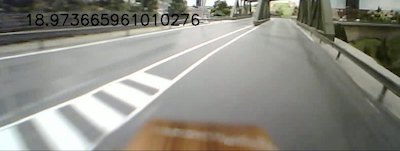
\includegraphics{Trainingsdaten-1}
					 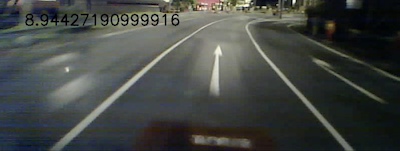
\includegraphics{Trainingsdaten-2}
					 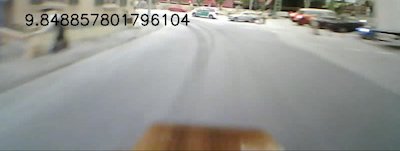
\includegraphics{Trainingsdaten-3}
  					  \caption{Beispiele aus den Trainingsdaten mit eingeblendeten Metadaten.}
 					   \label{fig:trainigsdaten}
				\end{figure}
				
				\subsubsection{Optimierung}
				Das Netzwerk wird dahingehend Trainiert die durchschnittlichen Quadratischen Abweichung (mse) zwischen dem Ergebnis des Netzes und den gemessenen Daten zum Lenkwinkel zu minimieren. Dies führt dazu, dass große Abweichungen besonders stark Gewichtet werden und kleinere nur geringer. 
		
	
		
	\bibliography{references}
	\bibliographystyle{alpha}
	\nocite{*}
	
\end{document}